%!TEX root = ../hr-paper.tex
\newpage
\section{Experiment} % (fold)
\label{sec:experiment}

This section will show by example how the segmented dataset is validated.  

% how the labels are used with our images to validate our images.
% IOU


\begin{figure}[ht]
  \centering
  \begin{subfigure}{0.25\textwidth}
    \centering
    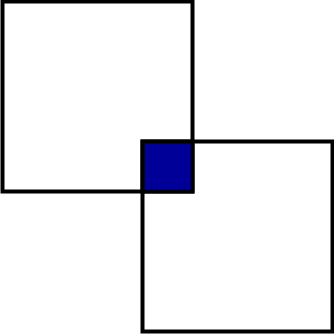
\includegraphics[width=\textwidth]{./images/experiment/intersection.png}
    \caption{Intersected area}
    \label{fig:experiment:intersection}
  \end{subfigure}
  \begin{subfigure}{0.25\textwidth}
    \centering
    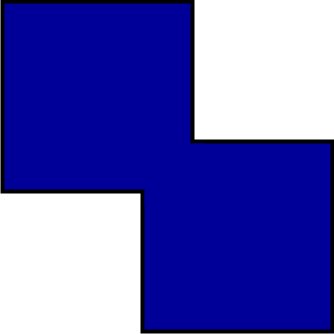
\includegraphics[width=\textwidth]{./images/experiment/union.png}
    \caption{Area of the union}
    \label{fig:experiment:union}
  \end{subfigure}
  \caption{Method of validating the segmented data (intersection over union)}
  \label{fig:experiment:iou}
\end{figure}

In order to validate the segmented images obtained by the segmentation the intersection over union is used. As shown in figure \ref{fig:experiment:intersection} the intersection between two boxes is the area that overlaps between these boxes. The union over two boxes give the area both the boxes occupy (figure \ref{fig:experiment:union}). The fraction between the intersection and the union tells us how well the boxes fit on top of each other. With this fraction the performance of the segmentation can be measured.

Because the characters consist mainly of black pixels, and the location of the box is arbitrary, the intersection over union is done only over the black pixels in both boxes. This is done by binerizing the original image and taking its complement. The complement is taken so black pixels will be represented by ones and white pixels by zeros. Now the labeled box and a segmented box are both printed on a white background the size of the original image. This results in two binary images on which an And is the same as the intersection, an Or is the same as a union. Summing the result from these operations give us the needed scalers to perform the intersection over union fraction.

 \begin{figure}[ht]
  \centering
  \begin{subfigure}{0.24\textwidth}
    \centering
    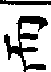
\includegraphics[width=0.7\textwidth]{./images/experiment/label.png}
    \caption{Label image}
    \label{fig:experiment:label}
  \end{subfigure}
  \begin{subfigure}{0.24\textwidth}
    \centering
    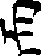
\includegraphics[width=0.7\textwidth]{./images/experiment/found.png}
    \caption{Segmented image}
    \label{fig:experiment:found}
  \end{subfigure}
    \begin{subfigure}{0.24\textwidth}
    \centering
    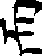
\includegraphics[width=0.7\textwidth]{./images/experiment/and.png}
    \caption{Label and Segmented}
    \label{fig:experiment:and}
  \end{subfigure}
  \begin{subfigure}{0.24\textwidth}
    \centering
    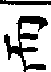
\includegraphics[width=0.7\textwidth]{./images/experiment/or.png}
    \caption{Label or Segmented}
    \label{fig:experiment:or}
  \end{subfigure}
  \caption{Example of intersection over union on a segmented character in the dataset, $IoU \approx 0.73$. The character used is the twelfth character in the image shown in figure \ref{fig:dataset:chinese:example}. }
  \label{fig:experiment:iou:example}
\end{figure}

In order to be able to say anything about the performance of the segmentation results will be thresholded from an intersection over union rate from 0.1 to 10. if the intersection over union is lower than 0.1 the boxes are not touching each other enough.


\subsection{Feature Extraction}

The feature extraction for the experiment was done in two variants: one dataset was generated with the Sobel filters and the other was generated with the use of the Prewit filters. This means that feature 21 (length) and 22 (width) are the same for both datasets. This was done one the segmented dataset created by the segmentation system and on the received labeled dataset.

\subsection{Classification}

Classification was done by taking the distance measure's described in the method section \todo{ref} and running the KNN algorithm with them. For the Minkowski measure, values from $p=1$ to $p=6$ were used. This experiment was run on the dataset normalized and non-normalized.

For the KNN algorithm $K=1$ to $K=5$ was used. Also all runs were done for $K=1$ to $K=100$ with all distance measures in order to see if a `large' $K$ has an unexpected influence on the classification results.

In order to gain the classification rates, the `leave one out' strategy was used. This strategy takes one data-point from the dataset and tries to classify it on the rest of the dataset. This is done for every point in the dataset. It is the extreme case of n-fold data splitting where the maximum number of splits is used.

For the LVQ methods a parameter sweep was done to find the best performing dataset with the best performing preprocessing. The parameter sweep was done with 2000 iterations on the segmented dataset with Sobel feature extraction. The dataset were prepared with three methods of preprocessing:

\begin{enumerate}
  \item No preprocessing (NONE)
  \item Feature columns normalized to values between one and zero (NORM)
  \item Feature columns normalized so the variation is between one and zero (VAR)
\end{enumerate}

When the best performing method is found, the best LVQ method will be run on all datasets with the best performing preprocessing. The number of max iterations will be set to 8000.
The LVQ methods were initialized with one prototype per class, These prototypes were initialized near the mean of their respectable classes. For LVQ 10-fold data splitting was used because `leave one out' was too time consuming.

% knn
%   -naive
%     -Mahalanobis (Since mahalanobis already scales the data)
%   -norm
%     -Euclidian

% lvq (all methods)
%   -naive
%   -norm
%   -var_norm


% section experiment (end)
